\section{Morfeas WEB MDAQ-if/Portal UI}

The ``Morfeas WEB MDAQ-if/Portal" can be accessed from the Morfeas WEB front page by the button with the identical label.
An example of the ``Morfeas WEB MDAQ-if/Portal UI" derived at figure \ref{fig:MDAQ-if_UI}.
At the top left corner are a drop down menu that can select the MDAQ component under interest, by it's defined name.\\

\noindent The ``Morfeas WEB MDAQ-if/Portal UI" split in three sections.
The to drop down menu that explained above, the status box, and the measurement table.
The status text box show the last update (fetch) date, or the last error that happens.
The measurement table on the upper side show the configuration of the component together with the temperature of the MDAQ board and the connection status.
The lower part contains that measurements that comes from the MDAQ.
Each one channel of the MDAQ provide three values. Each value have different meaning that related to the channel configuration.
The channels can be configured only (unfortunately) by a proprietary tool that given my the manufacture.

\begin{figure}[h]
\centering
	\fbox{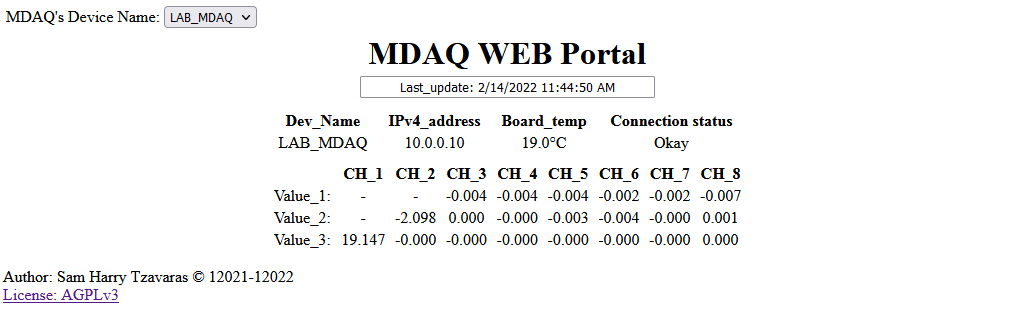
\includegraphics[width=5in,angle=0]{../art/Morfeas_web_if/Morfeas_web_MDAQ_if_UI.png}}
	\caption{Example of Morfeas WEB MDAQ-if UI}
	\label{fig:MDAQ-if_UI}
\end{figure}